\section{Z and t Statistics}

\begin{enumerate}
	\item Suppose that the parameter value assumed under the null hypothesis is $A_0$. 
	\item We take a random sample of 100 or 1000 individuals or instances of the event. 
	\item We calculate the sample mean of the parameter, for example the average age in a city, the mean pizza delivery time, the mean income, etc. 
	\item We denote this sample mean by $A$.
\end{enumerate}




The $Z$ statistic is calculated to transform a normally distributed random variable (for example, the sampling distribution of the population mean age) into a standard normal distribution.
%  This is because the probability values for a variable that follows the standard normal distribution can be obtained from a precalculated table.


The $Z$ statistic is given by the following formula:
\begin{align}
	\label{eq:3.6.1}
	Z=\dfrac{A-A_{0}}{{\sigma}/{\sqrt{n}}}
\end{align}
where $\s$ is the population standard deviation and $n$ is the number of observations in the sample.


Now, we must consider two cases:

\subsection{Z-Test (Normal Distribution)}
The researcher knows the population standard deviation of the parameter from past experience.



A good example of this is the case of pizza delivery times. In this case, \eqref{eq:3.6.1} will follow a normal distribution and the standardized values are known as \emph{Z-values}.

\subsection{t-Test (Student's t-Distribution)}
In this case, the researcher does not know the population standard deviation.



This can happen because:
\begin{itemize}
	\item Such data does not exist in historical records;
	\item or the number of events or individuals is too small to assume a normal distribution.
\end{itemize}


In this case, both the mean and standard deviation are unknown, and the expression follows a non-normal distribution called \emph{Student's $t$-distribution}.



The standardized value in this case is called a \emph{$t$-value} and the test is called a \emph{$t$-test}.


\subsection{Student's t-Distribution}
\begin{quote}
	The Student's $t$-distribution was described in 1908 by William Sealy Gosset. Gosset worked at the Guinness brewery, which prohibited its employees from publishing scientific articles due to the prior disclosure of industrial secrets. Hence, Gosset published his results under the pseudonym of "Student". \footnote{
		\href{https://en.wikipedia.org/wiki/Student\%27s_t-distribution\#History}{Wikipedia: Student's $t$-distribution}
	}
\end{quote}


\begin{figure}
	\centering
	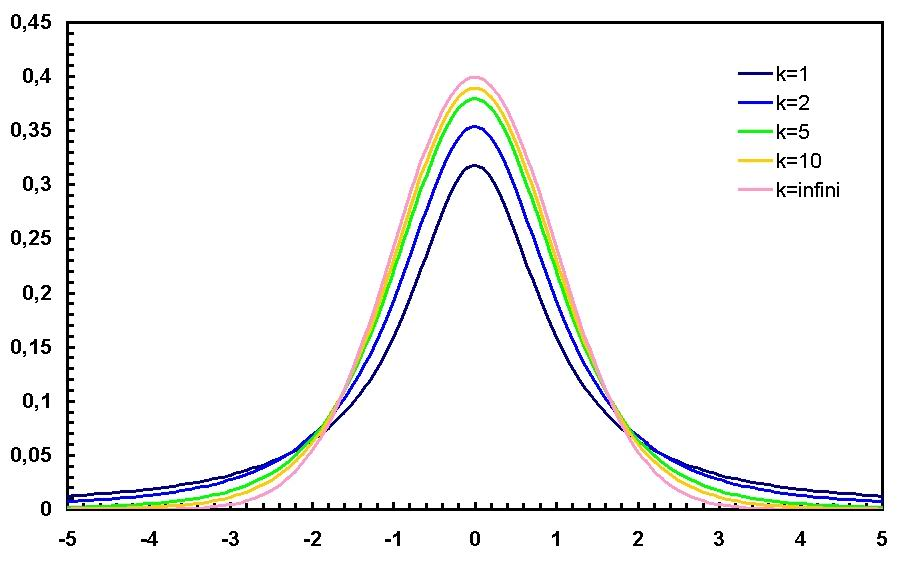
\includegraphics[height=5cm,keepaspectratio=true]{./images/Student_densite_best.jpg}
	% Student_densite_best.jpg: 0x0 pixel, 300dpi, 0.00x0.00 cm, bb=
	\caption{From The original uploader was Thorin on French Wikipedia - Transferred from fr.wikipedia to Commons., CC BY-SA 1.0, https://commons.wikimedia.org/w/index.php?curid=1878902}
	\label{fig:3.6.1}
\end{figure}




\begin{figure}
	\centering
	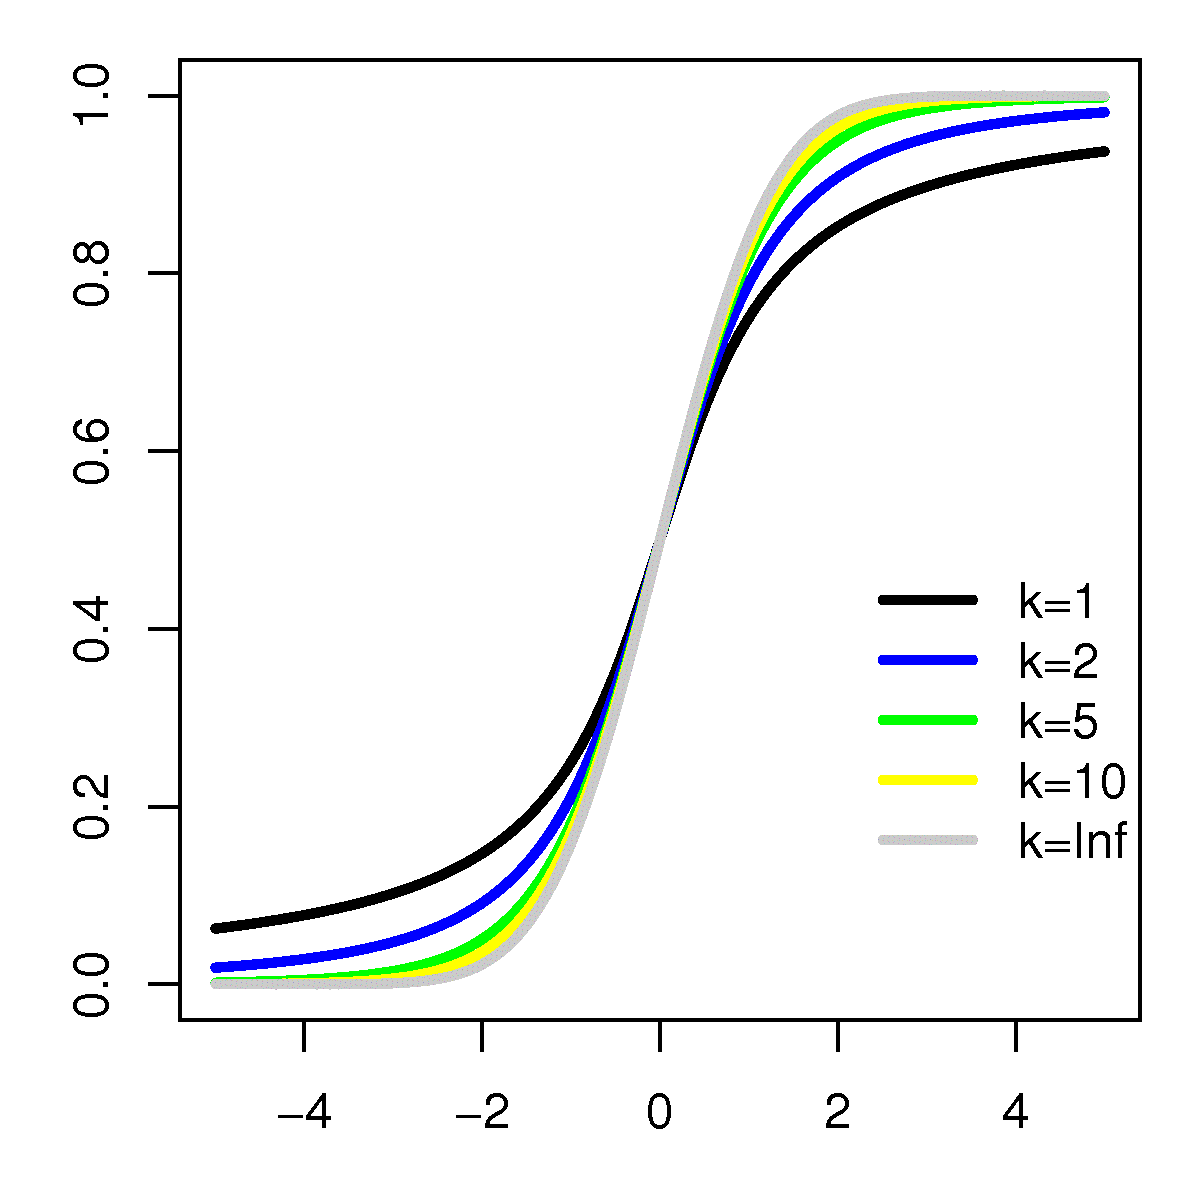
\includegraphics[height=5cm,keepaspectratio=true]{./images/T_distributionCDF.png}
	% T_distributionCDF.png: 0x0 pixel, 300dpi, 0.00x0.00 cm, bb=
	\caption{From Unknown, CC BY-SA 3.0, https://commons.wikimedia.org/w/index.php?curid=788691}
	\label{fig:3.6.2}
\end{figure}

\begin{lstlisting}[language=Python, caption=$t$-Distribution in \texttt{Python}]
	from scipy import stats
	import numpy as np
	import matplotlib.pyplot as plt
	
	def ft(x, nu):
	return stats.t.pdf(x, df=nu)
	def Ft(x, nu):
	return stats.t.cdf(x, df=nu)
	x = np.arange(-4,4,0.01)
	yd = ft(x,30)
	yc = Ft(x,30)
	
	fig, ax = plt.subplots()
	plt.plot(x, yd, 'r', linewidth=2)
	plt.plot(x, yc, 'b', linewidth=2)
	plt.ylim(ymin=0)
	plt.show()
\end{lstlisting}



\begin{figure}
	\centering
	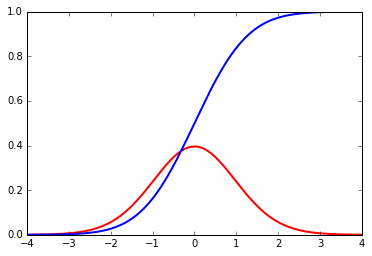
\includegraphics[height=7cm,keepaspectratio=true]{./images/tCDF.png}
	% tCDF.png: 0x0 pixel, 300dpi, 0.00x0.00 cm, bb=
\end{figure}



The \texttt{df} parameter is known as the \emph{degrees of freedom} and is generally denoted by $\nu$ (the Greek letter \texttt{nu}).


If a random variable $X$ has a $t$-distribution with $\nu$ degrees of freedom, then
\begin{align}
	\mu_{X}=0, \; \s^{2}_{X}=\dfrac{\nu}{\nu-2}
\end{align}



\begin{ejemplo}
	Consider a variable with a $t$-distribution and $\nu=9$ degrees of freedom. Find the value of $t$ for which the area to the right is $0.05$ but the total unshaded area is $0.90$.
	\begin{figure}
		\centering
		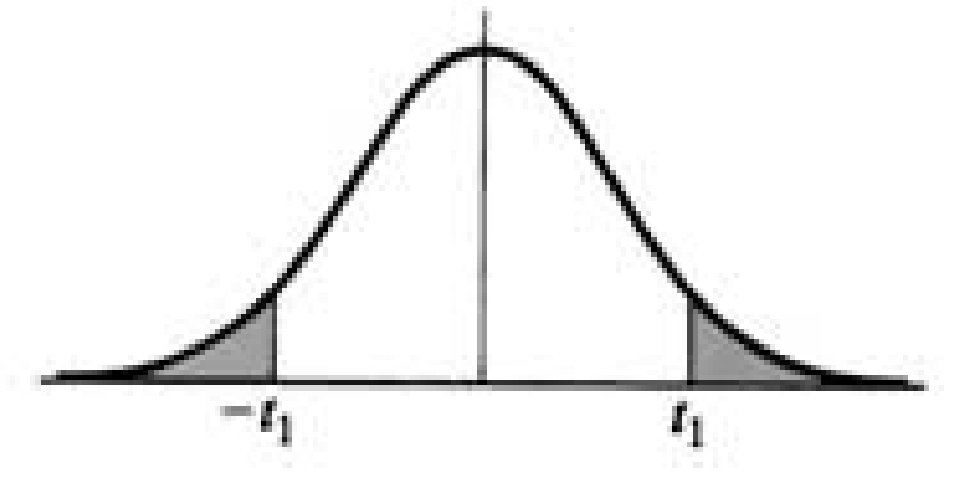
\includegraphics[height=3cm,,keepaspectratio=true]{./images/tExample.png}
		% tExample.png: 0x0 pixel, 300dpi, 0.00x0.00 cm, bb=
	\end{figure}
\end{ejemplo}

\begin{solucion}
	We seek the $t$-value such that the area to the right is $0.05$. This means that the area to the left is $1 - 0.05 = 0.95$.
	
	Using the percent point function (ppf) of the $t$-distribution with $\nu=9$ degrees of freedom:
	\begin{align}
		t_{0.05, 9} = t_{0.95} \approx 1.833
	\end{align}
	
	By symmetry of the $t$-distribution, the value that leaves an area of $0.05$ to the left is $-1.833$.
	
	The total unshaded area (between $-1.833$ and $1.833$) is:
	\begin{align}
		P(-1.833 < T < 1.833) = 0.95 - 0.05 = 0.90
	\end{align}
\end{solucion}


\begin{lstlisting}[language=Python]
	from scipy import stats
	import numpy as np
	import matplotlib.pyplot as plt
	
	def tp(x, nu):
		return stats.t.ppf(x, df=nu)
	
	print(tp(0.05, 9))
	##-1.83311293265
	print(tp(1-0.05, 9))
	##1.83311293265
\end{lstlisting}

\subsection{Sample Variance}
\begin{align}
	S^{2}=\sum\dfrac{\left( A_{i}-A_{0} \right)^{2}}{n-1}
\end{align}


\subsection{t-Statistic}
\begin{align}
	t = \dfrac{\left( A-A_{0} \right)}{S/\sqrt{n}}
\end{align}
